% Options for packages loaded elsewhere
% Options for packages loaded elsewhere
\PassOptionsToPackage{unicode}{hyperref}
\PassOptionsToPackage{hyphens}{url}
%
\documentclass[
  ignorenonframetext,
  aspectratio=169,
]{beamer}
\newif\ifbibliography
\usepackage{pgfpages}
\setbeamertemplate{caption}[numbered]
\setbeamertemplate{caption label separator}{: }
\setbeamercolor{caption name}{fg=normal text.fg}
\beamertemplatenavigationsymbolsempty
% remove section numbering
\setbeamertemplate{part page}{
  \centering
  \begin{beamercolorbox}[sep=16pt,center]{part title}
    \usebeamerfont{part title}\insertpart\par
  \end{beamercolorbox}
}
\setbeamertemplate{section page}{
  \centering
  \begin{beamercolorbox}[sep=12pt,center]{section title}
    \usebeamerfont{section title}\insertsection\par
  \end{beamercolorbox}
}
\setbeamertemplate{subsection page}{
  \centering
  \begin{beamercolorbox}[sep=8pt,center]{subsection title}
    \usebeamerfont{subsection title}\insertsubsection\par
  \end{beamercolorbox}
}
% Prevent slide breaks in the middle of a paragraph
\widowpenalties 1 10000
\raggedbottom
\AtBeginPart{
  \frame{\partpage}
}
\AtBeginSection{
  \ifbibliography
  \else
    \frame{\sectionpage}
  \fi
}
\AtBeginSubsection{
  \frame{\subsectionpage}
}
\usepackage{iftex}
\ifPDFTeX
  \usepackage[T1]{fontenc}
  \usepackage[utf8]{inputenc}
  \usepackage{textcomp} % provide euro and other symbols
\else % if luatex or xetex
  \usepackage{unicode-math} % this also loads fontspec
  \defaultfontfeatures{Scale=MatchLowercase}
  \defaultfontfeatures[\rmfamily]{Ligatures=TeX,Scale=1}
\fi
\usepackage{lmodern}

\ifPDFTeX\else
  % xetex/luatex font selection
\fi
% Use upquote if available, for straight quotes in verbatim environments
\IfFileExists{upquote.sty}{\usepackage{upquote}}{}
\IfFileExists{microtype.sty}{% use microtype if available
  \usepackage[]{microtype}
  \UseMicrotypeSet[protrusion]{basicmath} % disable protrusion for tt fonts
}{}
\makeatletter
\@ifundefined{KOMAClassName}{% if non-KOMA class
  \IfFileExists{parskip.sty}{%
    \usepackage{parskip}
  }{% else
    \setlength{\parindent}{0pt}
    \setlength{\parskip}{6pt plus 2pt minus 1pt}}
}{% if KOMA class
  \KOMAoptions{parskip=half}}
\makeatother


\usepackage{longtable,booktabs,array}
\usepackage{calc} % for calculating minipage widths
\usepackage{caption}
% Make caption package work with longtable
\makeatletter
\def\fnum@table{\tablename~\thetable}
\makeatother
\usepackage{graphicx}
\makeatletter
\newsavebox\pandoc@box
\newcommand*\pandocbounded[1]{% scales image to fit in text height/width
  \sbox\pandoc@box{#1}%
  \Gscale@div\@tempa{\textheight}{\dimexpr\ht\pandoc@box+\dp\pandoc@box\relax}%
  \Gscale@div\@tempb{\linewidth}{\wd\pandoc@box}%
  \ifdim\@tempb\p@<\@tempa\p@\let\@tempa\@tempb\fi% select the smaller of both
  \ifdim\@tempa\p@<\p@\scalebox{\@tempa}{\usebox\pandoc@box}%
  \else\usebox{\pandoc@box}%
  \fi%
}
% Set default figure placement to htbp
\def\fps@figure{htbp}
\makeatother


% definitions for citeproc citations
\NewDocumentCommand\citeproctext{}{}
\NewDocumentCommand\citeproc{mm}{%
  \begingroup\def\citeproctext{#2}\cite{#1}\endgroup}
\makeatletter
 % allow citations to break across lines
 \let\@cite@ofmt\@firstofone
 % avoid brackets around text for \cite:
 \def\@biblabel#1{}
 \def\@cite#1#2{{#1\if@tempswa , #2\fi}}
\makeatother
\newlength{\cslhangindent}
\setlength{\cslhangindent}{1.5em}
\newlength{\csllabelwidth}
\setlength{\csllabelwidth}{3em}
\newenvironment{CSLReferences}[2] % #1 hanging-indent, #2 entry-spacing
 {\begin{list}{}{%
  \setlength{\itemindent}{0pt}
  \setlength{\leftmargin}{0pt}
  \setlength{\parsep}{0pt}
  % turn on hanging indent if param 1 is 1
  \ifodd #1
   \setlength{\leftmargin}{\cslhangindent}
   \setlength{\itemindent}{-1\cslhangindent}
  \fi
  % set entry spacing
  \setlength{\itemsep}{#2\baselineskip}}}
 {\end{list}}
\usepackage{calc}
\newcommand{\CSLBlock}[1]{\hfill\break\parbox[t]{\linewidth}{\strut\ignorespaces#1\strut}}
\newcommand{\CSLLeftMargin}[1]{\parbox[t]{\csllabelwidth}{\strut#1\strut}}
\newcommand{\CSLRightInline}[1]{\parbox[t]{\linewidth - \csllabelwidth}{\strut#1\strut}}
\newcommand{\CSLIndent}[1]{\hspace{\cslhangindent}#1}



\setlength{\emergencystretch}{3em} % prevent overfull lines

\providecommand{\tightlist}{%
  \setlength{\itemsep}{0pt}\setlength{\parskip}{0pt}}



 


\makeatletter
\@ifpackageloaded{caption}{}{\usepackage{caption}}
\AtBeginDocument{%
\ifdefined\contentsname
  \renewcommand*\contentsname{Table of contents}
\else
  \newcommand\contentsname{Table of contents}
\fi
\ifdefined\listfigurename
  \renewcommand*\listfigurename{List of Figures}
\else
  \newcommand\listfigurename{List of Figures}
\fi
\ifdefined\listtablename
  \renewcommand*\listtablename{List of Tables}
\else
  \newcommand\listtablename{List of Tables}
\fi
\ifdefined\figurename
  \renewcommand*\figurename{Figure}
\else
  \newcommand\figurename{Figure}
\fi
\ifdefined\tablename
  \renewcommand*\tablename{Table}
\else
  \newcommand\tablename{Table}
\fi
}
\@ifpackageloaded{float}{}{\usepackage{float}}
\floatstyle{ruled}
\@ifundefined{c@chapter}{\newfloat{codelisting}{h}{lop}}{\newfloat{codelisting}{h}{lop}[chapter]}
\floatname{codelisting}{Listing}
\newcommand*\listoflistings{\listof{codelisting}{List of Listings}}
\makeatother
\makeatletter
\makeatother
\makeatletter
\@ifpackageloaded{caption}{}{\usepackage{caption}}
\@ifpackageloaded{subcaption}{}{\usepackage{subcaption}}
\makeatother

\usepackage{bookmark}
\IfFileExists{xurl.sty}{\usepackage{xurl}}{} % add URL line breaks if available
\urlstyle{same}
\hypersetup{
  pdftitle={Parte 1 : Regressão},
  hidelinks,
  pdfcreator={LaTeX via pandoc}}



\title{Parte 1 : Regressão}
\author{}
\date{}

\begin{document}
\frame{\titlepage}


\section{Introdução}\label{introduuxe7uxe3o}

\begin{frame}{O que é Aprendizagem?}
\phantomsection\label{o-que-uxe9-aprendizagem}
\begin{itemize}
\tightlist
\item
  \textbf{Definição de aprendizagem:} É uma mudança adaptativa no
  comportamento causada pela experiência.
\end{itemize}

\pause

\begin{itemize}
\tightlist
\item
  Praticamente todos os animais com sistema nervoso central são capazes
  de aprender (mesmo os mais simples).
\end{itemize}
\end{frame}

\begin{frame}{O que é Aprendizagem?}
\phantomsection\label{o-que-uxe9-aprendizagem-1}
\begin{itemize}
\tightlist
\item
  \textbf{O que significa para um computador aprender? Por que queremos
  que ele aprenda? Como fazemos para que ele aprenda?}

  \begin{itemize}
  \tightlist
  \item
    Queremos que computadores aprendam quando é muito difícil ou muito
    caro programá-los diretamente para executar uma tarefa.
  \item
    Fazemos o computador ``programar a si mesmo'' ao mostrar exemplos de
    entradas e saídas.

    \begin{itemize}
    \tightlist
    \item
      Na prática, escrevemos um programa ``parametrizado'' e deixamos
      que o algoritmo de aprendizagem encontre o conjunto de parâmetros
      que melhor aproxima a função ou o comportamento desejado.
    \end{itemize}
  \end{itemize}
\end{itemize}
\end{frame}

\begin{frame}{Definições Clássicas de Aprendizado de Máquina}
\phantomsection\label{definiuxe7uxf5es-cluxe1ssicas-de-aprendizado-de-muxe1quina}
\textbf{Arthur Samuel (1959):}

\begin{quote}
\emph{``Aprendizado de Máquina é o campo de estudo que dá aos
computadores a habilidade de aprender sem serem explicitamente
programados.''}
\end{quote}

\pause

\textbf{Tom Mitchell (1997):}

\begin{quote}
\emph{``Dizemos que um programa de computador aprende a partir de uma
experiência \(E\), com respeito a alguma tarefa \(T\) e alguma medida de
desempenho \(P\), se o seu desempenho na tarefa \(T\), medido por \(P\),
melhora com a experiência \(E\).''}
\end{quote}
\end{frame}

\begin{frame}{Definições Clássicas de Aprendizado de Máquina}
\phantomsection\label{definiuxe7uxf5es-cluxe1ssicas-de-aprendizado-de-muxe1quina-1}
\begin{itemize}
\tightlist
\item
  \textbf{\(T\) --- Task (Tarefa):} A tarefa que queremos resolver.

  \begin{itemize}
  \tightlist
  \item
    Exemplos:

    \begin{itemize}
    \tightlist
    \item
      classificar e-mails, prever preço de casas, detectar fraude
    \end{itemize}
  \end{itemize}
\end{itemize}

\pause

\begin{itemize}
\tightlist
\item
  \textbf{\(E\) --- Experience (Experiência):} Os dados utilizados para
  aprender.

  \begin{itemize}
  \tightlist
  \item
    Exemplo:

    \begin{itemize}
    \tightlist
    \item
      histórico de e-mails rotulados como \textbf{spam} ou \textbf{não
      spam}
    \end{itemize}
  \end{itemize}
\end{itemize}

\pause

\begin{itemize}
\tightlist
\item
  \textbf{\(P\) --- Performance (Desempenho):} Métrica usada para
  avaliar o modelo.

  \begin{itemize}
  \tightlist
  \item
    Exemplos:

    \begin{itemize}
    \tightlist
    \item
      acurácia, erro quadrático médio, AUC
    \end{itemize}
  \end{itemize}
\end{itemize}
\end{frame}

\begin{frame}{Por que precisamos de Aprendizado de Máquina?}
\phantomsection\label{por-que-precisamos-de-aprendizado-de-muxe1quina}
É muito difícil resolver problemas como o \textbf{reconhecimento de
objetos bidimensionais ou tridimensionais}.

\begin{itemize}
\item
  Não sabemos qual programa escrever, pois \textbf{não sabemos
  exatamente como o cérebro realiza essa tarefa}.
\item
  Mesmo que soubéssemos, \textbf{o programa provavelmente seria
  extremamente complexo}.
\end{itemize}
\end{frame}

\begin{frame}{Exemplo: reconhecimento de dígitos manuscritos}
\phantomsection\label{exemplo-reconhecimento-de-duxedgitos-manuscritos}
Um exemplo clássico é o reconhecimento automático de \textbf{dígitos
escritos à mão}.

A variabilidade na forma como cada pessoa escreve os números torna muito
difícil criar \textbf{regras explícitas de programação} para identificar
cada dígito.

Em vez disso, usamos \textbf{aprendizado de máquina}, que permite ao
algoritmo \textbf{aprender padrões diretamente a partir dos dados}.
\end{frame}

\begin{frame}{Exemplo: dígitos manuscritos (MNIST)}
\phantomsection\label{exemplo-duxedgitos-manuscritos-mnist}
\begin{center}

\includegraphics[width=0.85\linewidth,height=\textheight,keepaspectratio]{intro_files/figure-beamer/unnamed-chunk-1-1.png}
\end{center}
\end{frame}

\begin{frame}{Por que precisamos de Aprendizado de Máquina?}
\phantomsection\label{por-que-precisamos-de-aprendizado-de-muxe1quina-1}
\begin{block}{A abordagem de aprendizado de máquina}
\phantomsection\label{a-abordagem-de-aprendizado-de-muxe1quina}
Em vez de escrever um programa manualmente, coletamos \textbf{muitos
exemplos} que especificam a saída correta para uma determinada entrada.

Um \textbf{algoritmo de aprendizado de máquina} produz um programa a
partir desses dados.

\begin{itemize}
\item
  O programa produzido por um algoritmo de aprendizado pode ser
  \textbf{muito diferente de um programa típico escrito manualmente}.
\item
  Se fizermos isso corretamente, o programa \textbf{funciona para novos
  casos}, além daqueles usados no treinamento.
\end{itemize}
\end{block}
\end{frame}

\begin{frame}
\begin{block}{Observação importante}
\phantomsection\label{observauxe7uxe3o-importante}
{ Grandes quantidades de computação e dados hoje são mais baratas do que
pagar alguém para escrever um programa manualmente. }
\end{block}
\end{frame}

\begin{frame}{Programação Tradicional vs Aprendizado de Máquina}
\phantomsection\label{programauxe7uxe3o-tradicional-vs-aprendizado-de-muxe1quina}
\begin{block}{Programação tradicional}
\phantomsection\label{programauxe7uxe3o-tradicional}
Nós escrevemos explicitamente as regras.

{Entrada + Regras → Saída}

Exemplo:

\begin{itemize}
\tightlist
\item
  \textbf{Entrada:} dados de um cliente
\item
  \textbf{Regras:} lógica escrita pelo programador
\item
  \textbf{Saída:} decisão do sistema
\end{itemize}
\end{block}
\end{frame}

\begin{frame}
\begin{block}{Aprendizado de máquina}
\phantomsection\label{aprendizado-de-muxe1quina}
O algoritmo aprende as regras a partir dos dados.

{Entrada + Saída → Algoritmo → Modelo}

Exemplo:

\begin{itemize}
\tightlist
\item
  \textbf{Dados:} histórico de clientes
\item
  \textbf{Respostas:} compra / não compra
\item
  \textbf{Modelo aprendido:} sistema de previsão
\end{itemize}
\end{block}
\end{frame}

\begin{frame}{Diferentes Tipos de Aprendizado}
\phantomsection\label{diferentes-tipos-de-aprendizado}
\begin{block}{Aprendizado Supervisionado}
\phantomsection\label{aprendizado-supervisionado}
{Entrada → Saída conhecida}

Exemplos:

\begin{itemize}
\tightlist
\item
  classificação de imagens
\item
  previsão de preços
\item
  detecção de spam
\end{itemize}
\end{block}
\end{frame}

\begin{frame}
\begin{block}{Aprendizado Não Supervisionado}
\phantomsection\label{aprendizado-nuxe3o-supervisionado}
{Somente entradas disponíveis}

Objetivo:

\begin{itemize}
\tightlist
\item
  descobrir padrões ocultos
\item
  identificar grupos
\end{itemize}

Exemplos:

\begin{itemize}
\tightlist
\item
  \textbf{clusterização}
\item
  \textbf{redução de dimensionalidade}
\end{itemize}
\end{block}
\end{frame}

\begin{frame}
\begin{block}{Aprendizado por Reforço}
\phantomsection\label{aprendizado-por-reforuxe7o}
{Agente interage com um ambiente}

Componentes:

\begin{itemize}
\tightlist
\item
  \textbf{estado}
\item
  \textbf{ação}
\item
  \textbf{recompensa}
\end{itemize}

Exemplos:

\begin{itemize}
\tightlist
\item
  robôs
\item
  jogos
\item
  veículos autônomos
\end{itemize}
\end{block}
\end{frame}

\begin{frame}
\begin{center}
\pandocbounded{
\includegraphics[keepaspectratio]{intro_files/figure-beamer/unnamed-chunk-2-1.png}}
\end{center}
\end{frame}

\section{Aprendizado Supervisionado}\label{aprendizado-supervisionado-1}

\begin{frame}{Notação e Suposições}
\phantomsection\label{notauxe7uxe3o-e-suposiuxe7uxf5es}
No \textbf{aprendizado supervisionado}, dispomos de um conjunto de
treinamento:

\[
\{(x_1, y_1), (x_2, y_2), \ldots, (x_n, y_n)\}
\]

onde:

\begin{itemize}
\tightlist
\item
  \(x_i = (x_{i1}, \ldots, x_{id})\) representa as \textbf{variáveis
  explicativas}
\item
  \(y_i\) representa a \textbf{variável resposta observada}
\end{itemize}
\end{frame}

\begin{frame}
A partir dos dados de treinamento, queremos aprender uma função
\(f(\mathbf{x})\) capaz de prever a resposta para \textbf{novas
observações}.

\pause

👉 Quando \(Y\) é \textbf{quantitativa}, buscamos aproximar a
\textbf{função de regressão}

\[
f(\mathbf{x}) = \mathbb{E}[Y \mid X = \mathbf{x}]
\]

como forma de descrever a relação entre uma variável aleatória
\(Y \in \mathbb{R}\) e um vetor de variáveis explicativas
\(\mathbf{x} = (x_1, \ldots, x_p) \in \mathbb{R}^p\)
\end{frame}

\begin{frame}{Formulação do aprendizado estatístico}
\phantomsection\label{formulauxe7uxe3o-do-aprendizado-estatuxedstico}
Uma forma comum de representar o problema é

\[
Y = f(\mathbf{x}) + \varepsilon
\]

onde:

\begin{itemize}
\tightlist
\item
  \(f(\mathbf{x})\) é a \textbf{função verdadeira desconhecida}
\item
  \(\varepsilon\) representa \textbf{ruído aleatório}
\end{itemize}

O objetivo do \textbf{aprendizado supervisionado} é \textbf{estimar}
(treinar) uma aproximação

\[
\hat f(\mathbf{x}) \approx f(\mathbf{x})
\]
\end{frame}

\begin{frame}{Predição versus Inferência: Por que estimar f(x)?}
\phantomsection\label{prediuxe7uxe3o-versus-inferuxeancia-por-que-estimar-fx}
\begin{block}{Exemplo 1.1 --- Expectativa de vida e PIB per capita}
\phantomsection\label{exemplo-1.1-expectativa-de-vida-e-pib-per-capita}
Considere dados de \textbf{211 países no ano de 2012}, contendo:

\begin{itemize}
\tightlist
\item
  \textbf{PIB per capita}
\item
  \textbf{expectativa de vida}
\end{itemize}

Uma pergunta natural é:

\begin{quote}
Como podemos usar esses dados para \textbf{estabelecer uma relação entre
essas duas variáveis}?
\end{quote}
\end{block}
\end{frame}

\begin{frame}
\begin{block}{Objetivo}
\phantomsection\label{objetivo}
Queremos usar os dados para \textbf{estimar a expectativa de vida de um
país} quando seu \textbf{PIB per capita é conhecido}.

Formalmente, queremos estimar

\[
\mathbb{E}[Y \mid X = x]
\]

onde

\begin{itemize}
\tightlist
\item
  \(Y\) = expectativa de vida de um país
\item
  \(X\) = PIB per capita
\end{itemize}
\end{block}
\end{frame}

\begin{frame}
\begin{block}{Interpretação da função de regressão}
\phantomsection\label{interpretauxe7uxe3o-da-funuxe7uxe3o-de-regressuxe3o}
A quantidade

\[
\mathbb{E}[Y \mid X = x]
\]

representa a \textbf{expectativa de vida média esperada para países com
PIB per capita igual a \(x\)}.

Estimando essa função podemos:

\begin{itemize}
\tightlist
\item
  \textbf{prever expectativa de vida} a partir do PIB per capita
\item
  \textbf{investigar a relação entre as variáveis}
\item
  \textbf{testar a hipótese de que não existe relação entre elas}
\end{itemize}
\end{block}
\end{frame}

\begin{frame}
\pandocbounded{
\includegraphics[keepaspectratio]{intro_files/figure-beamer/unnamed-chunk-3-1.png}}
\end{frame}

\begin{frame}{Predição versus Inferência: Por que estimar f(x)?}
\phantomsection\label{prediuxe7uxe3o-versus-inferuxeancia-por-que-estimar-fx-1}
\begin{block}{Exemplo 1.2 --- Distância de uma galáxia até a Terra}
\phantomsection\label{exemplo-1.2-distuxe2ncia-de-uma-galuxe1xia-atuxe9-a-terra}
Na cosmologia, uma variável extremamente importante é o \textbf{desvio
para o vermelho} (\emph{redshift}) de uma galáxia.

Esse valor mede \textbf{quão distante a galáxia está da Terra}.
\end{block}
\end{frame}

\begin{frame}
\begin{block}{O problema}
\phantomsection\label{o-problema}
O \textbf{redshift} pode ser medido com grande precisão por meio de
\textbf{espectroscopia}.

No entanto:

\begin{itemize}
\tightlist
\item
  esse procedimento é \textbf{caro}
\item
  exige \textbf{muito tempo de observação}
\end{itemize}

Por isso, surge a seguinte pergunta:

\begin{quote}
Podemos estimar o \textbf{redshift} utilizando apenas \textbf{imagens
das galáxias}?
\end{quote}
\end{block}
\end{frame}

\begin{frame}
\begin{block}{Formulação como aprendizado supervisionado}
\phantomsection\label{formulauxe7uxe3o-como-aprendizado-supervisionado}
Considere uma amostra de treinamento

\[
(\mathbf{x}_1,Y_1),\ldots,(\mathbf{x}_n,Y_n)
\]

onde

\begin{itemize}
\tightlist
\item
  \(\mathbf{x}_i\) = imagem da \(i\)-ésima galáxia\\
\item
  \(Y_i\) = redshift medido por espectroscopia
\end{itemize}
\end{block}
\end{frame}

\begin{frame}
\begin{block}{Objetivo}
\phantomsection\label{objetivo-1}
Queremos estimar a \textbf{função de regressão}

\[
f(x)=\mathbb{E}[Y \mid X=\mathbf{x}]
\]

A partir dessa função podemos:

\begin{itemize}
\tightlist
\item
  prever o \textbf{redshift} de novas galáxias
\item
  estimar suas \textbf{distâncias até a Terra}
\end{itemize}
\end{block}
\end{frame}

\begin{frame}{Predição versus Inferência: Por que estimar f(x)?}
\phantomsection\label{prediuxe7uxe3o-versus-inferuxeancia-por-que-estimar-fx-2}
\begin{block}{Exemplo 1.3 --- Isomap Face Data}
\phantomsection\label{exemplo-1.3-isomap-face-data}
Neste conjunto de dados, proveniente de Tenenbaum, Silva, and Langford
(2000), o objetivo é estimar \textbf{a direção para a qual uma pessoa
está olhando}.

\begin{itemize}
\tightlist
\item
  \textbf{Resposta (\(Y\)):} direção do olhar\\
\item
  \textbf{Covariáveis (\(\mathbf{x}\)):} imagem da face da pessoa
\end{itemize}
\end{block}
\end{frame}

\begin{frame}
\begin{block}{Formulação do problema}
\phantomsection\label{formulauxe7uxe3o-do-problema}
Uma forma de resolver esse problema é estimar a \textbf{função de
regressão}

\[
f(x) = \mathbb{E}[Y \mid X = \mathbf{x}]
\]

utilizando uma amostra de treinamento

\[
(\mathbf{x}_1,Y_1),\ldots,(\mathbf{x}_n,Y_n)
\]

onde:

\begin{itemize}
\tightlist
\item
  \(\mathbf{x}_i\) = imagem da face do indivíduo\\
\item
  \(Y_i\) = direção do olhar
\end{itemize}
\end{block}
\end{frame}

\begin{frame}
\begin{block}{Predição em novas imagens}
\phantomsection\label{prediuxe7uxe3o-em-novas-imagens}
Depois de estimar a função \(f(\mathbf{x})\), podemos utilizá-la para

\begin{itemize}
\tightlist
\item
  prever a \textbf{direção do olhar} em novas imagens
\item
  inferir a variável resposta \(Y\) a partir das covariáveis
  \(\mathbf{x}\)
\end{itemize}

\textbf{Em outras palavras:}

{imagem da face \(\rightarrow\) modelo \(\rightarrow\) direção do olhar}
\end{block}
\end{frame}

\begin{frame}
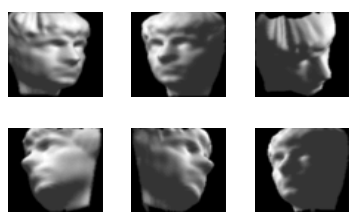
\includegraphics[width=10.41667in,height=\textheight,keepaspectratio]{../../../images/regressao/isomap_face.png}
\end{frame}

\begin{frame}{Predição versus Inferência: Por que estimar f(x)?}
\phantomsection\label{prediuxe7uxe3o-versus-inferuxeancia-por-que-estimar-fx-3}
\begin{block}{Exemplo 1.4 --- Predição do ano de lançamento de músicas}
\phantomsection\label{exemplo-1.4-prediuxe7uxe3o-do-ano-de-lanuxe7amento-de-muxfasicas}
Os dados do
\href{https://archive.ics.uci.edu/dataset/203/yearpredictionmsd}{\textbf{YearPredictionMSD}}
contêm diversas covariáveis sobre músicas do banco \textbf{Million Song
Dataset}.

Alguns exemplos de variáveis:

\begin{itemize}
\tightlist
\item
  características de \textbf{timbre}
\item
  \textbf{energia} da música
\item
  \textbf{dançabilidade}
\item
  outras características acústicas
\end{itemize}

Além disso, o conjunto de dados contém o \textbf{ano de lançamento} de
cada música.
\end{block}
\end{frame}

\begin{frame}
\begin{block}{Formulação como problema de regressão}
\phantomsection\label{formulauxe7uxe3o-como-problema-de-regressuxe3o}
Considere

\begin{itemize}
\tightlist
\item
  \(\mathbf{x}\) = vetor de características da música
\item
  \(Y\) = ano de lançamento
\end{itemize}

Queremos estimar a \textbf{função de regressão}

\[
f(x) = \mathbb{E}[Y \mid X = x]
\]

ou seja, o \textbf{ano esperado de lançamento dado o conjunto de
características da música}.
\end{block}
\end{frame}

\begin{frame}
\begin{block}{O que podemos fazer com esse modelo?}
\phantomsection\label{o-que-podemos-fazer-com-esse-modelo}
Uma estimativa de \(f(x)\) pode ser usada para:

\begin{enumerate}
\tightlist
\item
  \textbf{Predição}
\end{enumerate}

{Prever o ano de lançamento de novas músicas a partir de suas
características}

\begin{enumerate}
\setcounter{enumi}{1}
\tightlist
\item
  \textbf{Interpretação}
\end{enumerate}

{Investigar quais características musicais estão associadas ao ano de
lançamento}
\end{block}
\end{frame}

\begin{frame}
\begin{center}
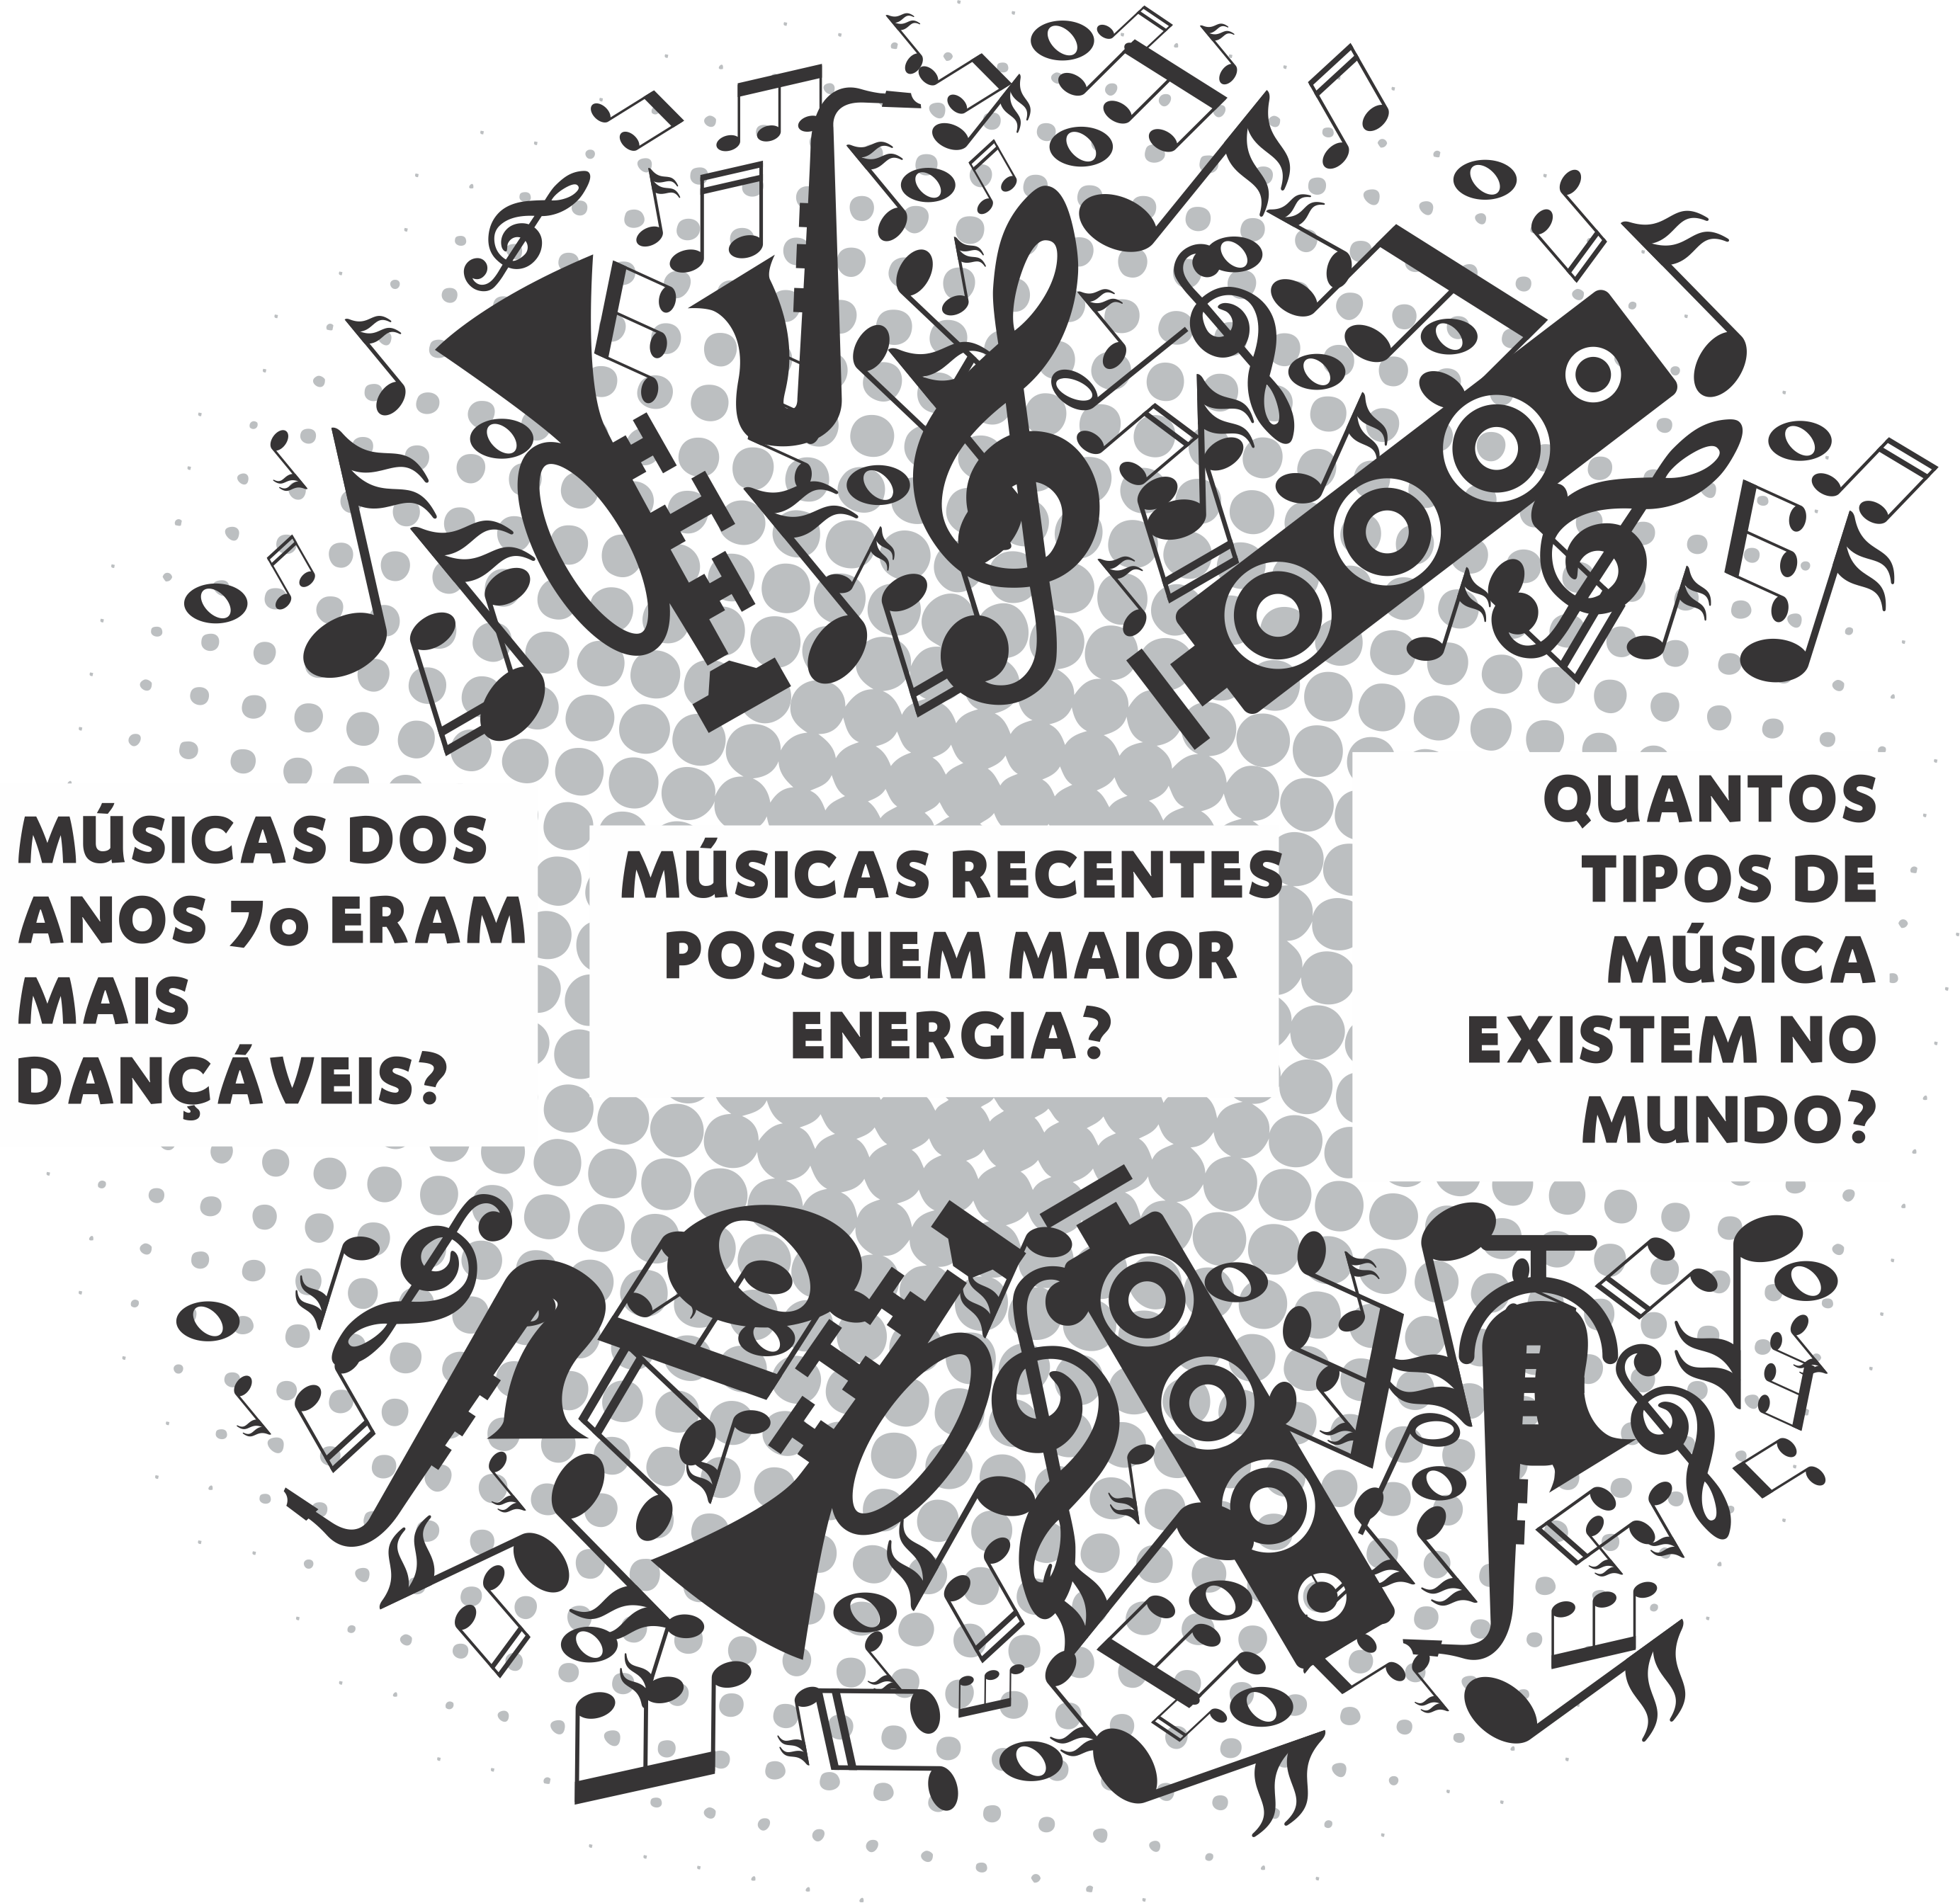
\includegraphics[width=0.4\linewidth,height=\textheight,keepaspectratio]{../../../images/regressao/tipos_musica.png}
\end{center}
\end{frame}

\begin{frame}
\begin{block}{Interpretação em aprendizado supervisionado}
\phantomsection\label{interpretauxe7uxe3o-em-aprendizado-supervisionado}
Temos uma amostra de treinamento

\[
(\mathbf{x}_1,Y_1),\ldots,(\mathbf{x}_n,Y_n)
\]

onde:

\begin{itemize}
\tightlist
\item
  \(\mathbf{x}_i\) = características da música
\item
  \(Y_i\) = ano de lançamento
\end{itemize}

O objetivo é aprender uma função

\[
\hat f(x)
\]

capaz de prever o \textbf{ano de lançamento de novas músicas}.
\end{block}
\end{frame}

\begin{frame}{Dois objetivos do aprendizado supervisionado}
\phantomsection\label{dois-objetivos-do-aprendizado-supervisionado}
De modo geral, os problemas apresentados podem ser divididos em
\textbf{dois objetivos principais}.

\begin{block}{Objetivo inferencial}
\phantomsection\label{objetivo-inferencial}
Perguntas típicas:

\begin{itemize}
\tightlist
\item
  Quais \textbf{preditores} são importantes?
\item
  Qual é a \textbf{relação entre cada preditor e a variável resposta}?
\item
  Qual é o \textbf{efeito de mudar o valor de um preditor} na variável
  resposta?
\end{itemize}

Esse tipo de análise busca \textbf{interpretar a relação entre as
variáveis}.
\end{block}
\end{frame}

\begin{frame}
\begin{block}{Objetivo preditivo}
\phantomsection\label{objetivo-preditivo}
Queremos construir uma função

\[
g : \mathbb{R}^d \rightarrow \mathbb{R}
\]

com \textbf{bom poder preditivo}.

A ideia é encontrar uma função \(g\) tal que, para novas observações
i.i.d.

\[
(X_{n+1},Y_{n+1}),\ldots,(X_{n+m},Y_{n+m}),
\]

tenhamos boas aproximações

\[
g(x_{n+1}) \approx y_{n+1}, \ldots, g(x_{n+m}) \approx y_{n+m}
\]
\end{block}
\end{frame}

\begin{frame}{Duas culturas em modelagem estatística}
\phantomsection\label{duas-culturas-em-modelagem-estatuxedstica}
Breiman (2001) argumenta que existem duas culturas no uso de modelos
estatísticos (em especial modelos de regressão).

\begin{block}{Data Modeling Culture}
\phantomsection\label{data-modeling-culture}
\begin{itemize}
\tightlist
\item
  Domina a \textbf{comunidade estatística}.
\item
  O principal objetivo está na \textbf{interpretação dos parâmetros}.
\item
  \textbf{Testar suposições do modelo} é fundamental.
\end{itemize}
\end{block}

\begin{block}{Foco:}
\phantomsection\label{foco}
\begin{itemize}
\tightlist
\item
  \textbf{Inferência}
\item
  Compreensão do mecanismo gerador dos dados
\end{itemize}
\end{block}
\end{frame}

\begin{frame}
\begin{block}{Algorithmic Modeling Culture}
\phantomsection\label{algorithmic-modeling-culture}
\begin{itemize}
\tightlist
\item
  Domina a \textbf{comunidade de Machine Learning}.
\item
  O foco está em \textbf{obter bons algoritmos preditivos}.
\item
  Os resultados podem ser interpretados, mas \textbf{isso geralmente não
  é o foco principal}.
\end{itemize}
\end{block}

\begin{block}{\textbf{Foco:}}
\phantomsection\label{foco-1}
\begin{itemize}
\tightlist
\item
  \textbf{Predição}
\item
  Desempenho em novos dados
\end{itemize}
\end{block}
\end{frame}

\begin{frame}{Integração entre Estatística e Machine Learning}
\phantomsection\label{integrauxe7uxe3o-entre-estatuxedstica-e-machine-learning}
\begin{quote}
\textbf{Machine Learning e Estatística não são opostos: são
complementares.}
\end{quote}

Historicamente, as duas áreas enfatizaram objetivos diferentes:

\begin{itemize}
\tightlist
\item
  \textbf{Estatística:} foco em \textbf{inferência e interpretação} dos
  modelos.
\item
  \textbf{Machine Learning:} foco em \textbf{predição e desempenho em
  novos dados}.
\end{itemize}
\end{frame}

\begin{frame}
\begin{block}{Tendência atual}
\phantomsection\label{tenduxeancia-atual}
Hoje muitos métodos modernos procuram \textbf{combinar as duas
culturas}, buscando:

\begin{itemize}
\tightlist
\item
  \textbf{alto desempenho preditivo}
\item
  \textbf{interpretação dos modelos}
\end{itemize}

Exemplos:

\begin{itemize}
\tightlist
\item
  \textbf{Random Forest interpretável}
\item
  \textbf{SHAP (Shapley Additive Explanations)}
\item
  \textbf{modelos semiparamétricos:} GAM (Modelos aditivos
  generalizados), Modelo de Cox (riscos proporcionais), etc.
\end{itemize}
\end{block}
\end{frame}

\begin{frame}
\begin{center}
\pandocbounded{
\includegraphics[keepaspectratio]{intro_files/figure-beamer/unnamed-chunk-4-1.png}}
\end{center}
\end{frame}

\begin{frame}{References}
\phantomsection\label{references}
\phantomsection\label{refs}
\begin{CSLReferences}{1}{0}
\bibitem[\citeproctext]{ref-breiman2001twocultures}
Breiman, Leo. 2001. {``Statistical Modeling: The Two Cultures.''}
\emph{Statistical Science} 16 (3): 199--231.
\url{https://doi.org/10.1214/ss/1009213726}.

\bibitem[\citeproctext]{ref-tenenbaum2000isomap}
Tenenbaum, Joshua B., Vin de Silva, and John C. Langford. 2000. {``A
Global Geometric Framework for Nonlinear Dimensionality Reduction.''}
\emph{Science} 290 (5500): 2319--23.
\url{https://doi.org/10.1126/science.290.5500.2319}.

\end{CSLReferences}
\end{frame}




\end{document}
